\newpage
\appendix
\appendixpage
\addappheadtotoc


\section{Key specifications}

\begin{table}[htbp]
   \centering
   \caption{Specifications Verification Matrix}
   \label{table:specifications-verification-matrix}
   \begin{tblr}{
      width=0.9\linewidth,
      colspec={|X|X|},
      hlines,
   }
   Specification & Verification \\
   \hline
   Train a policy in an empty world & Robot can reach the target position \\
   Train a policy in an indoor environment filled with obstacles & Robot can reach the target position and not collide with obstacles \\
   Trained policy can be used in unseen environment & Robot tries to move to the target while avoiding obstacle in an unexperienced environment \\
   \end{tblr}
\end{table}


\section{Gantt chart}
\label{appendix:gantt}

\begin{figure}[htbp]
   \centering
   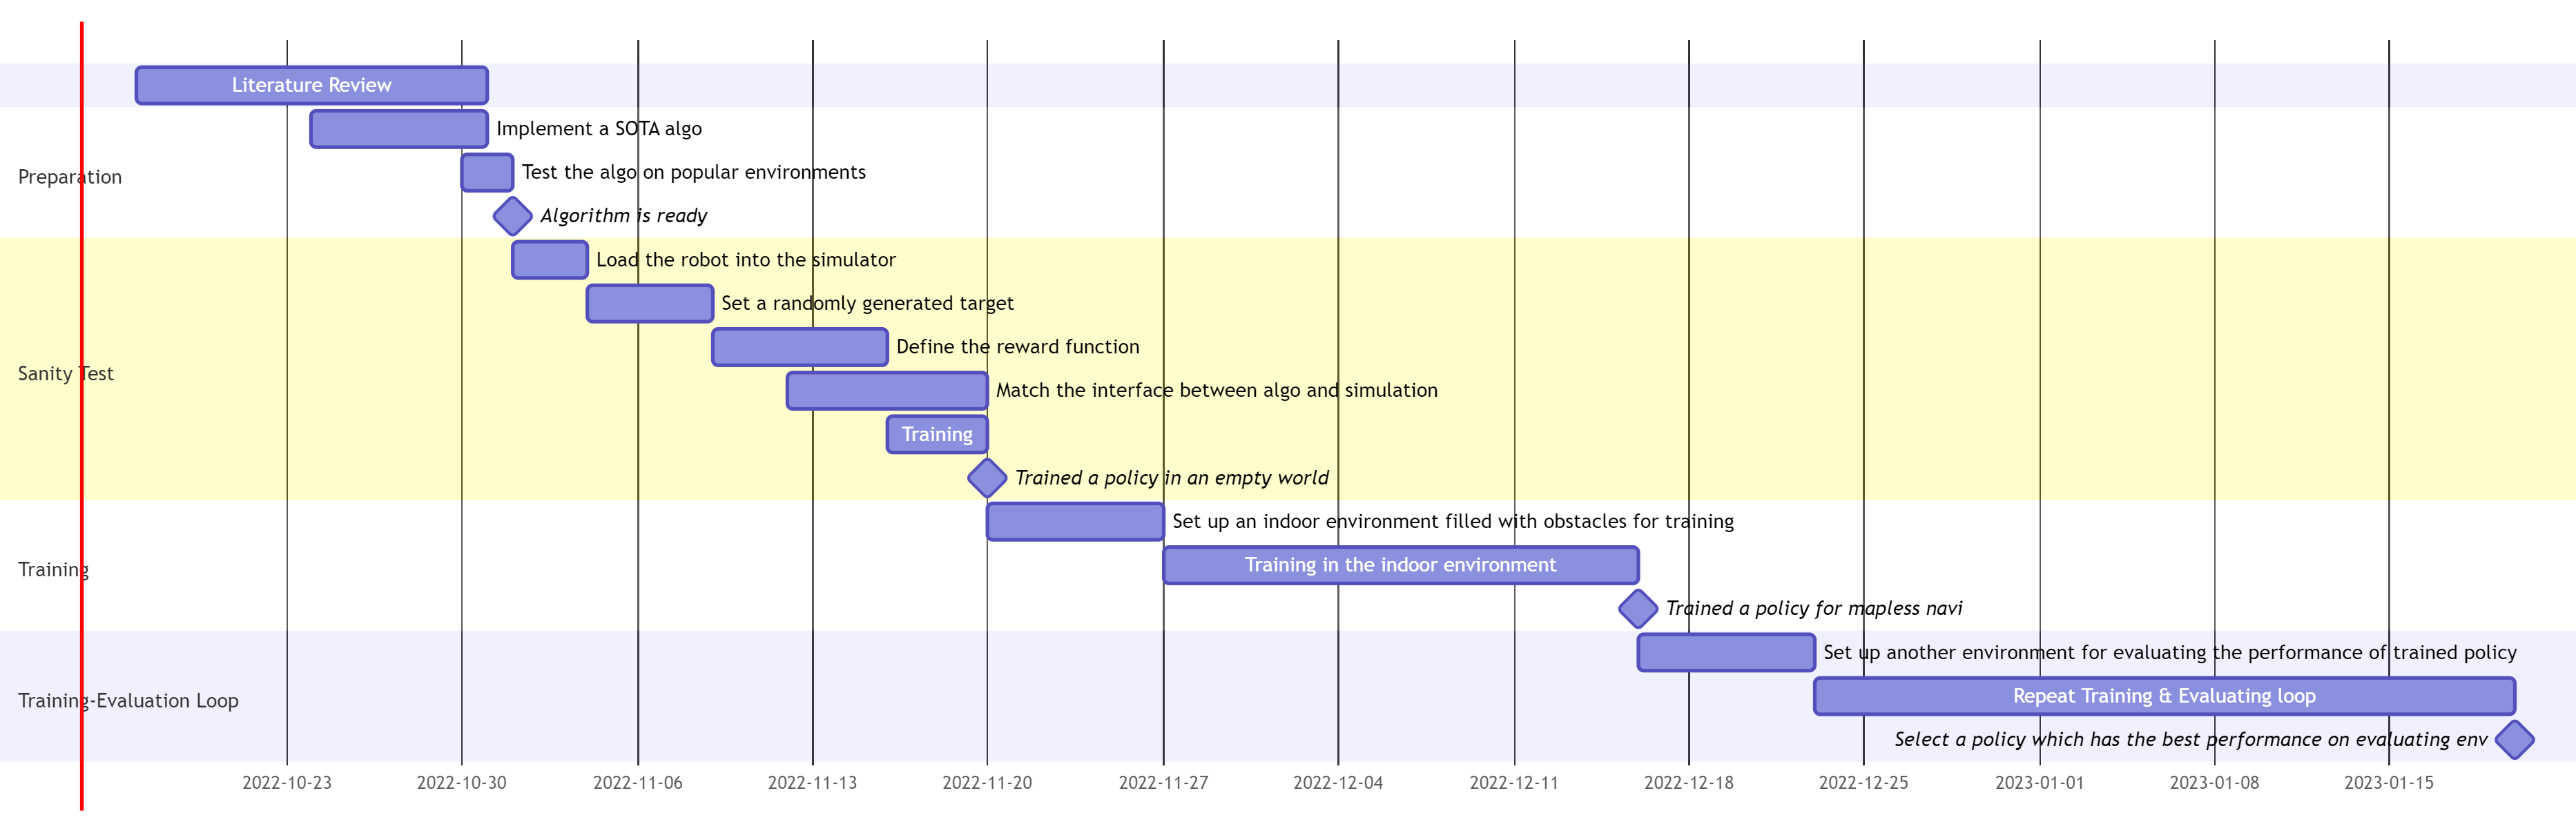
\includegraphics[width=\textwidth]{gantt}
   \caption{Gantt Chart}
   \label{fig:gantt}
\end{figure}


\section{List of work packages, milestones, and deliverables}
\label{appendix:tasks-milestones-deliverables}

\begin{itemize}
\item Literature review on mapless navigation with DRL.
\item Implement one of the SOTA DRL algo (PPO/TD3/SAC) in one week.
\item Train a policy in an empty world, four weeks before the end of the semester one.
\item Set up an indoor simulation environment filled with obstacles for training in one week.
\item Train a policy in the indoor environment, by the end of semester one.
\item Set up another environment for evaluating the performance of the trained policy in unseen environment in one week.
\item Train and evaluate the policy and select one which has the best performance in the evaluating environment, by the end of the project.
\item Design the poster and prepare the demo for bench inspection.
\item Document findings along the way in the final project report.
\end{itemize}


\section{Risk assessment form}
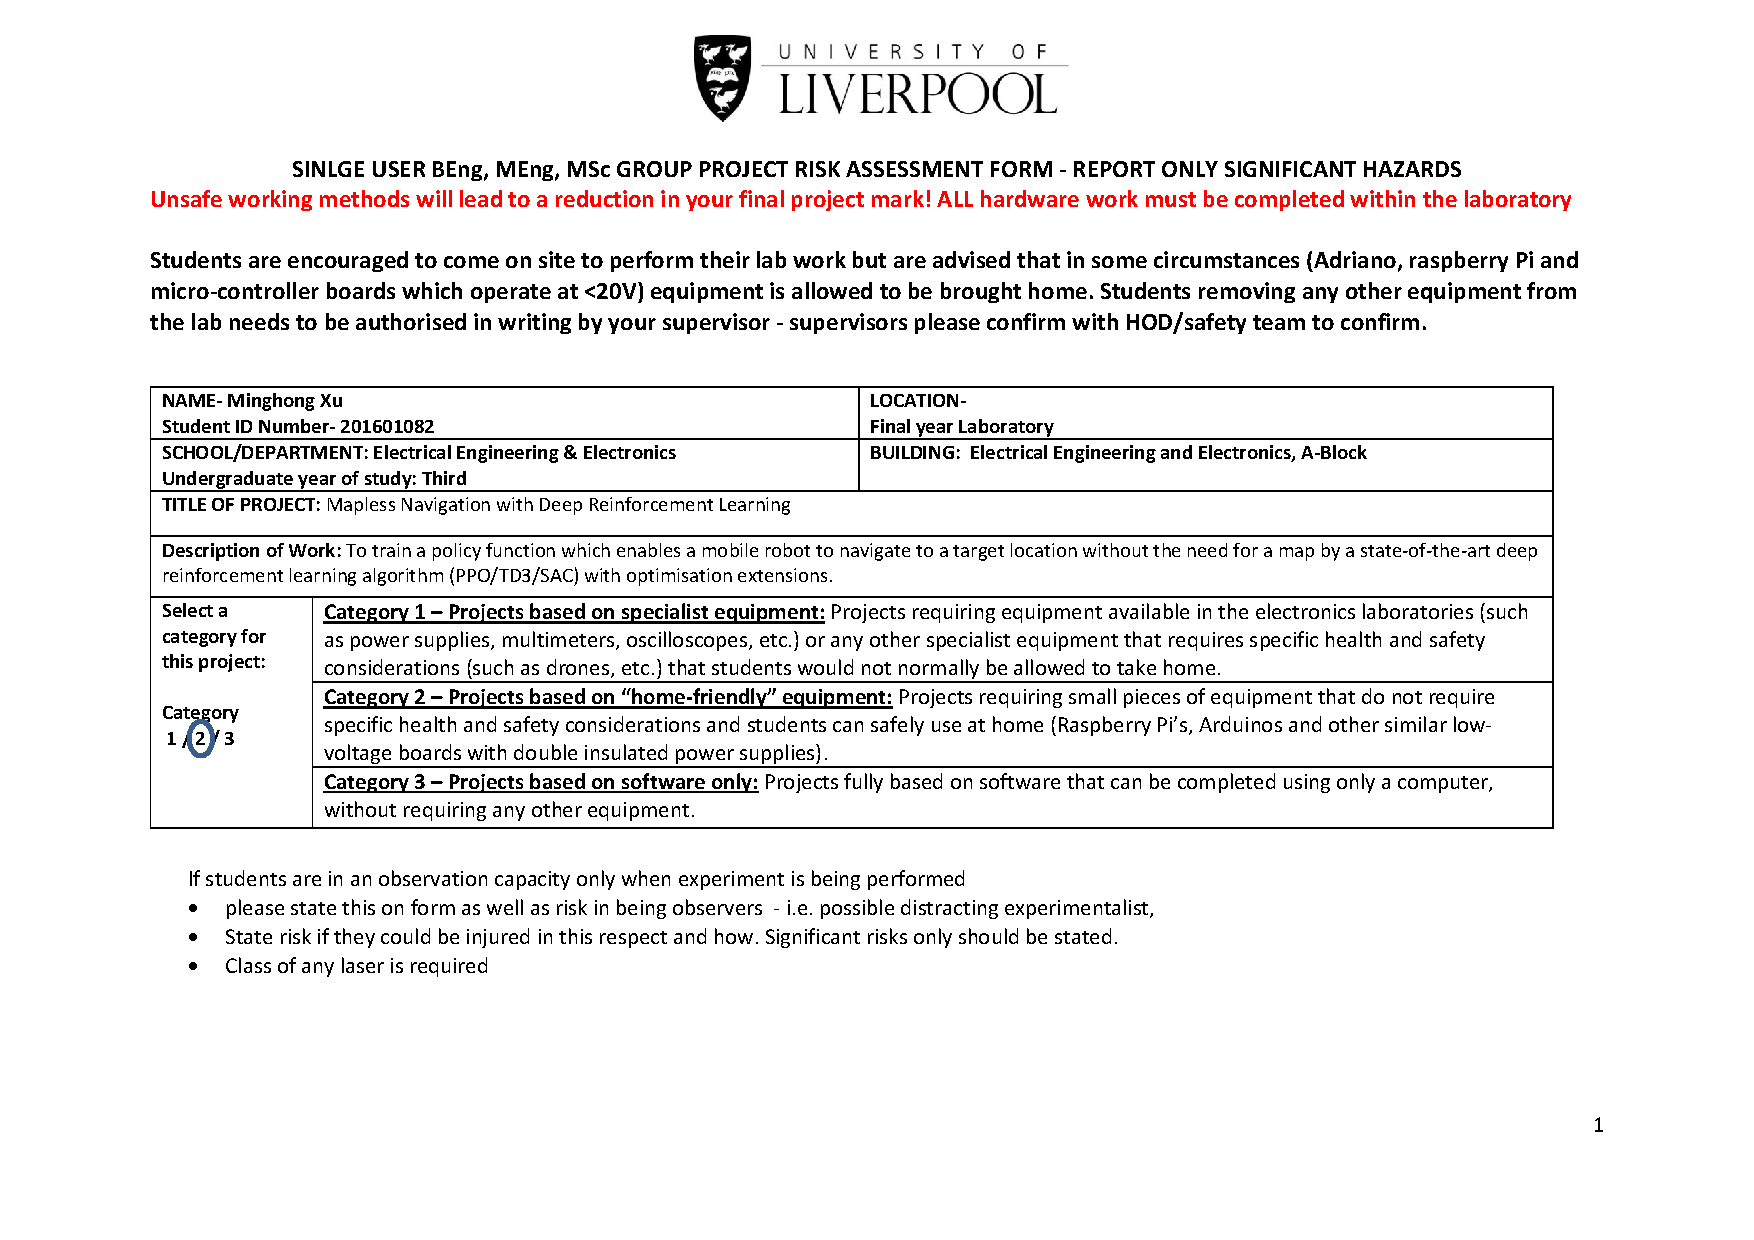
\includepdf[pages=-,fitpaper]{assets/risk-assessment-form.pdf}


\section{Ethical approval questionnaire}

\begin{figure}[htbp]
   \centering
   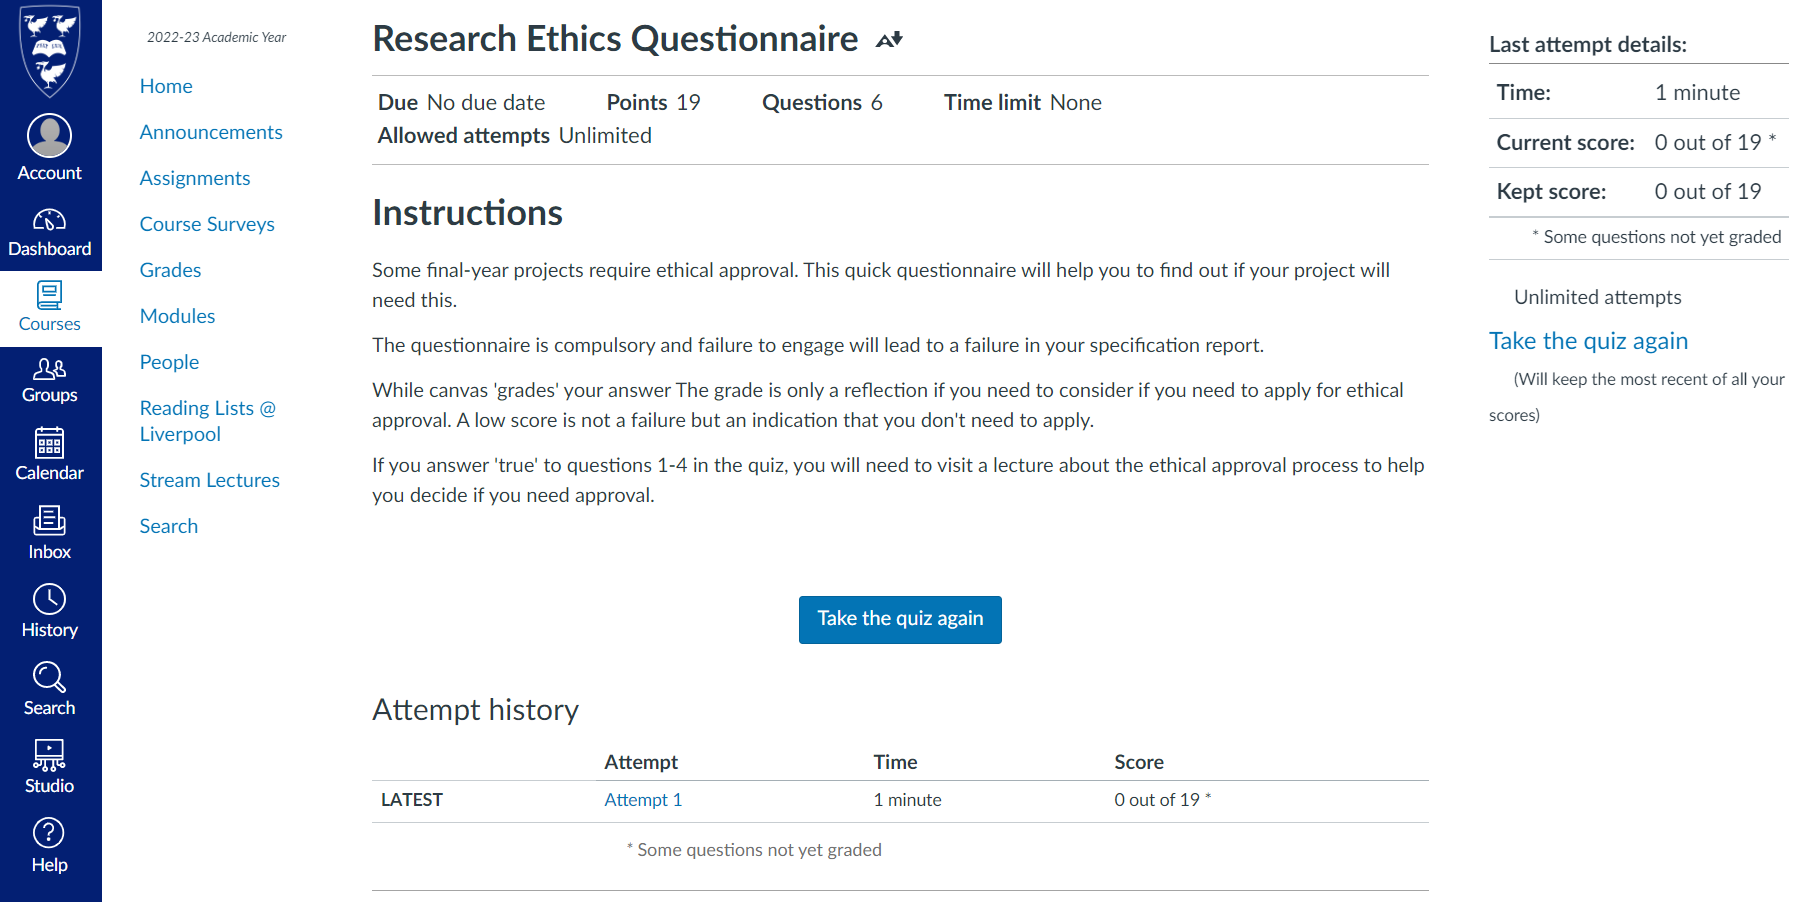
\includegraphics[width=0.85\textwidth]{ethics-questionnaire}
   \caption{Screenshot of completion of Ethics Questionnaire}
   \label{fig:ethics-questionnaire}
\end{figure}

